\documentclass[a4paper, 11pt, oneside]{report}

\usepackage[italian]{babel}
\usepackage[utf8]{inputenc}
\usepackage{hyperref}
\usepackage{amsmath}
\usepackage{listings}
\usepackage{graphicx}
\usepackage{dirtree}
\graphicspath{ {./img/} }
\usepackage{longtable}
\usepackage[toc,page]{appendix}

\title{Report progetto}
\author{Valentina Ceoletta VR407794\\Mattia Zanotti VR411086\\Nicol\`o Zenari VR412613}
\date{26 settembre 2018}

\begin{document}
\maketitle
\tableofcontents

\chapter{Descrizione del progetto}
Il progetto consiste nell'esplorare il web con l'obiettivo di raccogliere codice JavaScript considerato malevolo. In linea generale, il progetto inizia attraverso la collezione degli URL considerati malevoli dalla comunità \textit{hpHosts}. In secondo luogo, tali indirizzi web sono passati a \textit{heritrix}, un crawler in grado di effettuare il download delle pagine web e di tutte le risorse necessarie. Successivamente, i siti web scaricati con successo, vengono utilizzati come base per interrogare \textit{Virtus Total} e \textit{Google Safe Browsing}, due tool online in grado di fornire informazioni legate all'essere malevolo o meno. Il linguaggio scelto per completare il progetto è Python, un linguaggio ad alto livello semplice, flessibile e adatto alla realizzazione di script.
 
\section{File di configurazione} \label{sec:configFile}
All'interno della directory principale del progetto è presente il file \textit{config.json}, un file in cui sono strutturate tutte le informazioni necessarie per il corretto funzionamento del progetto. Di seguito, per ogni configurazione segue la spiegazione dell'utilizzo:
\begin{itemize}
	\item{\textit{out\_dir\_path}}: il path della directory in cui salvare tutte le risorse ottenute;
	\item{\textit{hosts\_dir\_path}}: directory in cui andranno salvate tutte le risorse di ogni host scaricato;
	\item{\textit{heritrix\_dir\_path}}: il nome della directory in cui lo script \textit{warcExtractor} crea le directory degli host;
	\item{\textit{javascript\_dir\_path}}: il nome della directory in cui lo script \textit{jsExtractor} salva i file javascrit estratti;
	\item{\textit{GSB\_dir}}: directory in cui vengono i creati i file \textit{bodyX.josn} necessari per interrogare Google Safe Browsing;
	\item{\textit{hosts\_json\_filename}}: nome del file JSON prodotto dallo script \textit{getHosts} contenente tutti gli host ottenuti da HpHosts con le relative informazioni;
	\item{\textit{seeds\_filename}}: nome del file prodotto dallo script  \textit{getHosts} contenente, riga per riga, l'URL degli host ottenuti da HpHosts;
	\item{\textit{host\_file\_url}}: URL di HpHosts (il parametro 0 indica la classe, mentre 1 indica la pagina);
	\item{\textit{download\_from\_date}}: data di pubblicazione da cui iniziare il download;
	\item{\textit{download\_to\_date}}: data di pubblicazione entro il quale terminare il download;
	\item{\textit{vt\_requests\_url}}: URL di VirusTotal necessario per inviare la richiesta;
	\item{\textit{vt\_report\_url}}: URL di VirusTotal necessario per ottenere il report;
	\item{\textit{vt\_api\_key}}: chive API di VirusTotal;
	\item{\textit{class\_to\_download}}: array di classi di HpHosts d'interesse;
	\item{\textit{json\_GSB\_filename}}: nome del file JSON necessari allo script \textit{gsb};
	\item{\textit{GSB\_url}}: URL di Google Safe Browsing;
	\item{\textit{GSB\_key}}: chiave API di Google Safe Browsing;
	\item{\textit{GSB\_clientId}}: nome dell'azienda (obbligatorio) per la richiesta a GSB;
	\item{\textit{GSB\_clientVersion}}: versione del client Google Safe Browsing;
    \item{\textit{GSB\_threatTypes}}: array di minacce (parametro di interrogazione di GSB);
    \item{\textit{GSB\_platformTypes}}: array di piattaforme (parametro di interrogazione di GSB);
    \item{\textit{GSB\_threatEntryTypes}}: tipologie ti entry passate a GSB attraverso i file JSON definiti in \textit{json\_GSB\_filename};
    \item{\textit{last\_check}}: ultimo controllo eseguito dallo scirpt \textit{getHosts}.
\end{itemize}


\section{getHosts}
Lo script \textit{getHosts} si occupa di richiedere e parserizzare le pagine HTML fornite da HpHosts con l'obiettivo di ottenere gli host desiderati. HpHosts è una repository di URL ritenuti malevoli da una comunità che viene aggiornata quotidiamente. Tra tutti gli host pubblicati sul sito, si è deciso di scaricare solo quelli che rientrano nella categoria \textbf{EMD}. La tipologia d'interesse viene specificata nel file di configurazione e più precisamente nell'array \textit{class\_to\_download}, mentre il periodo temporale necessario viene specificato agendo sulle variabili \textit{download\_from\_date}, \textit{download\_to\_date} e \textit{last\_check}. 

Lo script scarica la prima pagina solamente per ricavare il numero totale di pagine. Una volta ottenuta l'informazione, sulla base dei core disponibili nella macchina, vengono create tante thread quante il numero di core. Ogni thread ha il compito di interrogare e parserizzare tutte le pagine il cui numero è multiplo della prima pagina indicata (ad esempio, se si utilizzano 2 thread, la prima dovrà lavorare con le pagine 1,3,5,7, etc mentre la seconda con le pagine 2,4,6,8, etc).

Per quanto riguarda la parserizzazione, lo script estrapola la tabella HTML in cui sono contenuti tutti gli hosts. Per ogni host la cui classe corrisponde a una tra quelle desiderate, estrapola hostname, IP, classe, data di pubblicazione su hpHosts e data di aggiunta. Tutti gli host creati sono aggiunti ad una lista utile per la scrittura su file.

Ogni thread, come accennato precedentemente, si occupa di richiedere la pagina HTML e di parserizzarla in modo da estrapolare tutte le informazioni utili. Esse terminano se finiscono le pagine di loro competenza o se in una pagina è presente almeno un host già trattato \footnote{La data dell'ultimo controllo è specificata nel file di configurazione sotto la voce \textit{last\_check}}  oppure la cui data di pubblicazione è antecedente o seguente il periodo d'interesse.

Per ogni host che soddisfa le condizioni specificate nel file di configurazione, lo script \textit{hostInfo} invocato dalle thread di \textit{getHosts} si occupa di creare la seguente struttura ad albero delle directory con i relativi file di competenza:\\
\dirtree{%
.1 out.
.2 hosts.
.3 hostname1.
.4 info.json.
.3 hostname2.
.4 info.json.
.3 ....
}\label{dir}

\subsection{Output}
Il risultato dello script è:
\begin{itemize}
\item la directory di output;
\item la directory hosts;
\item una directory per ogni host;
\item il file \textit{info.json} all'interno della rispettiva cartella di ogni host.
\end{itemize}	

\subsection{Tempi di esecuzione}
I fattori che incidono sul tempo di esecuzione dello script sono \textbf{(1)} il numero di core messi a disposizione dal computer che si utilizza e \textbf{(2)} il numero di host che si vanno a scaricare in quanto il tempo impiegato da \textit{hpHosts} per creare una pagina è all'incirca di 3/5 secondi.

\section{Crawler}
Il crawler è un software che analizza i contenuti di una rete in modo metodico e automatizzato, si potrebbe definire un \textit{bot} che acquisisce una copia testuale di tutti i documenti visitati (HTML principalmente) e le salva in un file di output. Dalle recensioni web e dai giudizi degli utenti, utilizziamo Heritrix \cite{heritrix} nella versione 3.1.1 come crawler. Essendo altamente automatizzato è possibile impostare i parametri a piacimento nel file di configurazione \textit{crawler-beans.cxml}. Per il nostro obiettivo sono stati modificati i seguenti campi per poter estrarre solo le pagine utili:
\begin{itemize}
\item \textbf{org.archive.modules.seeds.TextSeedModule}: impostato per estrarre gli host da visitare dal file \textit{seeds.txt}, collocato nella directory principale del \textsf{jobs};
\item \textbf{org.archive.module.deciderules.DecideRuleSequence}: applicate una serie di regole in cascata tra cui: 
\begin{enumerate}
\item rifiuto di tutte le pagine
\item accetazione delle sole pagine \textsc{HTML} e \textsc{JS}
\item accettazione delle sole pagine a profondità 1 \textsf{hops} dal dominio principale;
\end{enumerate}
\item \textbf{org.archive.modules.Extractor}: applicazione dei soli estrattori \textsc{HTTP}, \textsc{HTML} e \textsc{JS};
\item \textbf{org.archive.modules.writer.WARCWriterProcessor}: salvataggi del crawling nel formato \textit{.warc};
\end{itemize}

La scelta della profondità è stata dettata dal fatto che outlink a potenziali pagine  o a potenziali script malevoli non sono raggiungibili con un numero di hop prefissati. Abbiamo deciso quindi di estrarre tutte le pagine \textsc{HTML} e \textsc{JavaScript} del dominio e poi le relative pagine collegate. Non tutti i siti permettono il crawling del proprio dominio, infatti Heritrix è stato impostato per non violare le direttive del file \textit{robots.txt} in cui vengono specificati dagli amministratori del sito, quali path sono accessibili e quali no. Alcuni vietano il completo crawling, perciò è possibile che alcuni host non vengano scaricati con successo ma ritornino un codice di errore relativo (per la lista completa visitare il seguente link: \url{https://github.com/internetarchive/heritrix3/wiki/Status%20Codes}). 
L'avvio del crawler avviene dapprima da linea di comando: 
\begin{lstlisting}[language=Bash]
$HERITRIX_HOME/bin/heritrix -a utente:password
\end{lstlisting}
e successivamente recandosi tramite web browser alla seguente pagina \\ \textsf{https://localhost:8443}. Si seleziona il job corrispondente \footnote{Si possono creare diversi job personalizzandoli a piacere}, si compila il crawler e poi lo si avvia premendo il bottone relativo.L'output che ne deriva è un file di tipo warc.gz.  \\

Tale file viene elaborato attraverso lo script Python \textit{warcExtractor.py}. Utilizzando un tool per l'estrazione delle informazioni dal file \textit{.warc} \cite{warc} , per ogni host scaricato con successo lo script crea una directory nominata \textit{heritrix} all'interno della cartella dell'host (vedi \ref{dir}) in cui salvare tutti i file associati. Per i siti in cui non è stato possibile il crawling, lo script provvederà a rimuoverne la directory creata in precedenza da \textit{getHosts}. Come ultimo lavoro, tutti gli host la cui operazione di raccolta è stata conclusa con successo verranno inseriti nel file \textit{seeds.txt} necessario a VirusTotal ed infine invocherà lo script \textit{hostInfo} per creare i file \textit{bodyN.json} necessari al modulo GSB.

Dopo la creazione delle directory, si avvia lo script Python \textit{jsExtractor.py} che provvede a creare una sub-directory \textsf{javascript} se è presente del codice \textsc{JavaScript} all'interno delle pagine scaricate.
Per poter estrarre il codice contenuto all'interno del tag $\langle\textsf{script}\rangle $ viene utilizzata la libreria \textit{BeautifulSoup} che fornisce dei metodi per la ricerca del tag desiderato all'interno del documento e ritorna la lista del contenuto. Tutte le parti di script o referenze a script esterni alla pagina vengono salvati in un unico file dal nome progressivo \textit{scriptN.js} all'interno della sub-directory creata precedentemente.\\

\subsection{Tempi di esecuzione}
I fattori che incidono sul tempo di esecuzione dello script sono \textbf{(1)} il numero di thread impostate nel crawler per poter scansionare la rete \textbf{(2)} il numero di host da visitare \textbf{(3)} il numero di host scaricati con successo dai quali estrarre i file associati \textbf{(4)} il quantitativo di codice javascript incluso nelle pagine scaricate

Al primo avvio il numero di host sarà certamente nell'ordine delle migliaia e il crawler richiede molte ore di processamento. Ai successivi avvii il tempo si accorcia.

\section{Google Safe Browsing (GSB)}
Uno script Python si occupa di interrogare Google Safe Browsing \cite{gsb} utilizzando il file \textit{bodyN.json}. Tali file si trovano seguendo il seguente albero:
\dirtree{%
.1 out.
.2 hosts.
.2 gsb.
.3 body0.json.
.3 body1.json.
.3 ....
}
 
L'implementazione della creazione di più file è stata necessaria in quanto Google impone l'interrogazione di al più 500 host per volta. All'interno dei Json sono contenute le seguenti informazioni:
\begin{itemize}
	\item \textit{ClientInfo}: le informazioni sul client che esegue la Safe Browsing API request;
	\item \textit{threatTypes}: il tipo di minaccia che si vuole controllare;
	\item \textit{platformTypes}: quali piattaforme controllare;
	\item \textit{threatEntryTypes}: il formato delle minacce che si vogliono analizzare (url, executable);
	\item \textit{threatEntries}: lista delle minacce da analizzare.
\end{itemize}
Il server di GSB esegue il join tra \textit{threatTypes}, \textit{platformTypes} e \textit{threatEntryTypes} ritornando quindi un file Json con molte voci ripetute. L'output viene quindi semplificato, indicando per ogni URL, le piattaforme per il quale risulta essere malevolo (es. Linux, Windows, OSX, \ldots) e il tipo di tipo di minaccia rilevata (Social Engineering, Malware, \ldots). Infine, tutte le informazioni ottenute sono salvate nel file \textit{gsb-tags.json} 

\subsection{Tempi di esecuzione}
Il tempo di esecuzione di Google Safe Browsing non allunga i tempi totali dell'intero progetto. L'esecuzione è nell'ordine di qualche secondo.

\section{Virus Total (VT)}
Lo script Python interroga Virus Total \cite{vt} utilizzando le sue API pubbliche. Virus Total nella sua versione gratuita è un servizio che analizza file sospetti o URLs e ne permette la rapida identificazione ed etichettatura. Dapprima si analizza il file \textit{seeds.txt} che contiene tutti gli hosts da verificare, poi si effettua la richiesta divisa nel seguente modo:
\begin{enumerate}
	\item una richiesta \textbf{post http} al server contenente l'url da analizzare;
	\item dopo l'analisi è necessaria una richiesta di \textbf{report} contenente un serie di informazioni; verrà applicato in secondo luogo un filtro per la selezione di solamente alcuni dati:
	\begin{itemize}
		\item \textit{vt\_scan\_date}: la data in cui è stata fatta la scansione su VT;
		\item \textit{positives}: il numero di antivirus che hanno riconosciuto l'URL analizzato come malevolo;
		\item \textit{total}: il numero complessivo di antivirus che hanno analizzato l'URL.
	\end{itemize}	 
\end{enumerate} 
Viene salvato tutto nel file \textit{vt-tags.json}. 

\subsection{Tempi di esecuzione}
Utilizzando le API pubbliche e gratuite di Virus Total è possibile fare al più 4 richieste al minuto, quindi è possibile analizzare al massimo 2 siti al minuto dato che ogni sito necessita di due chiamate al server.

\section{Statistiche}
\subsection{Google Safe Browsing}
Per lanciare le statistiche in merito alla quantità di host che Google Safe Browsing è riuscito a taggare è sufficiente lanciare lo script \textit{gsbStata}. Ogni host viene taggato solamente se sui server vengono trovate le informazioni necessarie. 

Dal 13 al 31 Agosto 2018, su 288 host collezionati, Google Safe Browsing ha taggato con successo 11 host. 

\subsection{Virus Total}
Per lanciare le statistiche in merito alla quantità di host che Virus Total ha classificato come non malevolo, è necessario lanciare lo script \textit{vtStata}. Ogni hosts verrà fatto analizzare da un serie di antivirus, ottenendo alla fine una percentuale sul riconoscimento dell'host come malevolo, ovvero Virus Total indicherà quanti antivirus hanno riconosciuto l'host come malevolo e il numero di  antivirus che hanno analizzato l' host.

Dal 13 al 31 Agosto 2018, su 288 host collezionati, Virus Total ha contrassegnato come non malevoli 51 host.

\subsection{eval}
Per lanciare le statistiche relative agli eval, è necessario lanciare lo script \textit{evalStata}.

Dal 13 al 31 Agosto 2018, con 288 host collezionati, sono stati prodotti 4494 file javascript. Di questi 5 presentano eval espliciti e 4489 contengono eval impliciti.
La statistica degli eval per singoli host si può trovare in \ref{tabella}.

\section{Schema del progetto}
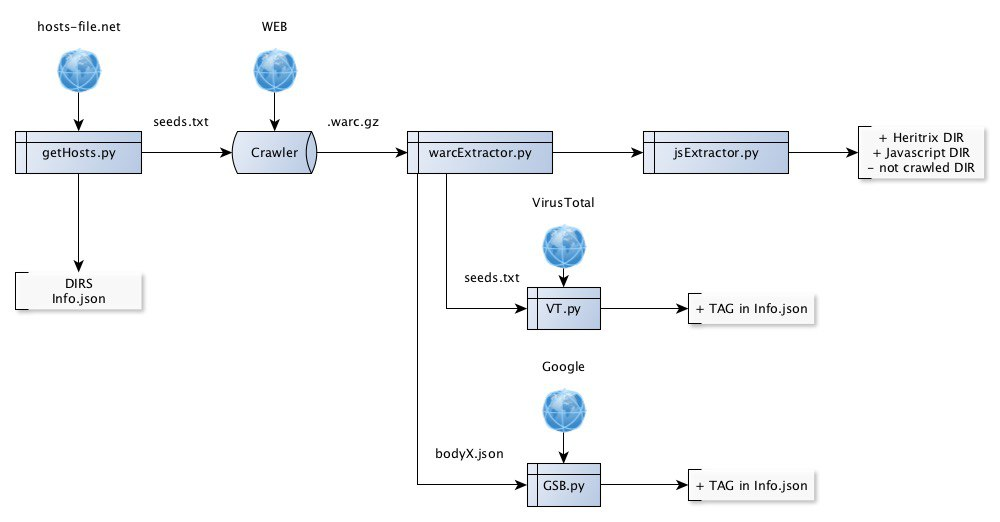
\includegraphics[scale=0.7]{schema}

\chapter{Appendice}
\section{Tabella eval per host}\label{tabella}
\begin{longtable}[!ht]{|l|c|c|}
    \hline
    \textbf{Host} & \textbf{Eval espliciti} & \textbf{Eval impliciti}  \\
    \hline
   	www.j610033.myjino.ru&0&3\\
\hline
www.veryaffordableblinds.com&0&3\\
\hline
sigtap.datasus.gov.br&0&4\\
\hline
rahulacollegeoba.lk&0&98\\
\hline
xhcrab.com&0&54\\
\hline
www.buyisraeli.co.il&0&45\\
\hline
pharezconsulting.com&0&2\\
\hline
www.mgprogramming.net&0&15\\
\hline
j.kyryl.ru&0&2\\
\hline
www.pset.ltd&0&2\\
\hline
www.tabanway.com.tr&0&227\\
\hline
steamdesktopauthenticator.com&0&2\\
\hline
www.gruzolub.ru&0&202\\
\hline
www.valoneew.beget.tech&0&3\\
\hline
pureleisurefun.com&0&121\\
\hline
plus.google.com&3&0\\
\hline
www.youtube.com&0&102\\
\hline
omexturviajes.com&0&22\\
\hline
twitter.com&0&407\\
\hline
www.hugedomains.com&0&42\\
\hline
www.smithmillie21.000webhostapp.com&0&2\\
\hline
hsa.ddns.net:8181&0&2\\
\hline
drclaudiadiez.com&0&1\\
\hline
nailedglamour.com&0&2\\
\hline
kaymanlimited.com&0&8\\
\hline
prijzen-dakkapel.nl&0&1\\
\hline
ajax.googleapis.com&0&1\\
\hline
infrarotgrill-test.info&0&3\\
\hline
wxklsb.com&0&57\\
\hline
dev2.mywebproof.net&0&9\\
\hline
zionsifac.com&0&23\\
\hline
cointradingsoftware.com&0&1\\
\hline
demo.proteusthemes.com&0&20\\
\hline
koenig-kebap.de&0&6\\
\hline
www2.datasus.gov.br&1&0\\
\hline
cosmos.cmitik.ru&0&5\\
\hline
mail.thuoht.website&0&3\\
\hline
www.rntk-imperia.ru&0&31\\
\hline
sites.google.com&0&5\\
\hline
mister-clean.pro&0&2\\
\hline
www.unimedmissoes.com.br&0&1\\
\hline
www.000webhost.com&0&169\\
\hline
www.sscgd.win&0&1\\
\hline
yarbisalama.hopto.org&0&1\\
\hline
hospitalsantoangelo.com&0&198\\
\hline
mypointapp.com&0&1\\
\hline
mac10mincomercio.000webhostapp.com&0&76\\
\hline
jaju.ltd&0&3\\
\hline
www.xhcrab.com&0&2\\
\hline
yawzee.me&0&4\\
\hline
www.collateralproduccions.com&0&1\\
\hline
www.st.is&0&10\\
\hline
kiyanka.club&0&3\\
\hline
www.clinicasaoangelo.com.br&0&3\\
\hline
piezodoorphone.com&0&29\\
\hline
windows10portal.com&0&47\\
\hline
www.ysd63.com&0&1450\\
\hline
www.smtechsrnc.com&0&1\\
\hline
br.wordpress.org&0&14\\
\hline
rahulacollege.org&0&27\\
\hline
www.secured-production.000webhostapp.com&0&2\\
\hline
www.cmitik.ru&0&4\\
\hline
centralappdownloadtrials.com&0&5\\
\hline
www.oxbourn.com&0&7\\
\hline
www.wxklsb.com&0&2\\
\hline
octopuspackaging.com&0&125\\
\hline
www.taverna-stuttgart.de&0&28\\
\hline
ideaintl.net&0&8\\
\hline
kassconnect.ru&0&77\\
\hline
www.zionsifac.com&0&1\\
\hline
ip01reg.myjino.ru&0&3\\
\hline
logs.icu&0&1\\
\hline
www.ipe.rs.gov.br&0&3\\
\hline
www.tulsamassageboutique.com&0&1\\
\hline
www.initex.com&0&1\\
\hline
houswe.com&0&223\\
\hline
www.google.com&0&6\\
\hline
cartaonet.datasus.gov.br&0&1\\
\hline
www.milfcamsluts.com&0&1\\
\hline
istanbuliklimlendirme.net&0&1\\
\hline
imagic-box.com&0&220\\
\hline
www.alvaro.com.br&0&34\\
\hline
kd.mestving.co.uk&0&1\\
\hline
www.cjoint.com&0&7\\
\hline
www.brcsari.ir&0&1\\
\hline
pratimspizza.com&0&145\\
\hline
www.nathaliedodon.com&1&2\\
\hline
\end{longtable}


\bibliographystyle{plain}
\bibliography{bibl}
\end{document}